\chapter{The stack}
\label{ch:the-stack}

\epigraph{\textit{}}{}

%--- --- --- --- --- --- --- --- --- --- --- --- --- --- --- --- ---
\section{When errors go wrong differently}
\label{sec:13:hook}
%--- --- --- --- --- --- --- --- --- --- --- --- --- --- --- --- ---

When you mishear a word, you usually mishear it as another word. You hear \mention{grape} as \mention{great}, not as a smear of sound. The perceptual system delivers discrete candidates, even when the input is noisy.

But when you mishear a sentence, something different happens. You might get every word right and still get the meaning wrong. \mention{The horse raced past the barn fell} is acoustically clear; the failure is structural. Or you hear the structure fine but miss the implicature: \mention{Some students passed} registers as good news when the speaker meant it as bad.

Why does error work differently at different scales?

The answer, this chapter argues, is that the \term{coupling regime} changes. At the sound level, form and function are so tightly bound that you can only err within the system---one phoneme for another, one word for another. At higher levels, form and function come apart enough that you can get one right and the other wrong.

This is the insight behind the ``stack'' metaphor. From phonemes to constructions to discourse, linguistic categories are homeostatic property clusters maintained by mechanisms. But the mechanisms differ, and so does the tightness of the form--function binding. What's invariant is the \emph{explanatory strategy}: when something behaves category-like, ask what stabilises the covariance and what it projects to. What varies is the \emph{stabiliser weighting}---which mechanisms dominate, and how transparent the coupling is.

The framework applies two diagnostics at each level. \term{Projectibility} asks whether patterns learned from one dataset can predict another---can we infer properties of new instances from old ones? \term{Homeostasis} asks whether we can name mechanisms that maintain the property cluster and identify their signatures in the data. These tests are independent. A category might project reliably without any identifiable mechanisms (overfitting to spurious patterns), or it might have plausible mechanisms that don't actually produce stable clustering (broken homeostasis). Both tests have to pass for kindhood to be warranted.

\subsection{What this chapter will show}

If the HPC framework applies at a new level, we expect to find:
\begin{enumerate}
    \item Properties that cluster without being definitionally linked.
    \item Mechanisms that maintain the clustering.
    \item Graded category membership at the boundaries.
    \item Historical mutability: perturbation degrades the cluster.
\end{enumerate}

These are the diagnostics. The chapter applies them to three positive cases (phonemes, morphemes, constructions) and three negative cases (academic register, ``Indo-European,'' ``polysynthetic''). The positive cases show the framework scaling. The negative cases show it has teeth---it can say \emph{no} as well as \emph{yes}.

One caveat before we begin. The tiers I'll discuss---phoneme, morpheme, construction, register---are convenient labels, not universal strata. They describe how English (and languages of similar type) organises its categories. Other languages draw the boundaries differently. A polysynthetic language blurs the morpheme--word line; an isolating language thins the morpheme tier almost to nothing; a click language reorganises phonetic space. The HPC explanatory strategy is domain-general. The stack is language-specific.

%--- --- --- --- --- --- --- --- --- --- --- --- --- --- --- --- ---
\section{The limit case: phonemes}
\label{sec:13:phonemes}
%--- --- --- --- --- --- --- --- --- --- --- --- --- --- --- --- ---

Say the word \mention{key}. Now say \mention{ski}. You probably think the /k/ sound is the same in both. It isn't.

In \mention{key}, your tongue is further forward, anticipating the front vowel. In \mention{ski}, it's further back. A spectrogram would show you: the burst frequencies differ, the formant transitions differ. They're acoustically distinct.

But you'll never hear the difference, because English doesn't care. Both sounds are filed under /k/. The phoneme is an abstraction over the acoustics---a category that groups variant tokens and opposes them to other categories (/g/, /t/, /p/).

This is what I mean by \term{transparent coupling}. At the phoneme level, form \emph{is} function. The acoustic pattern directly discharges the contrastive job without any intervening representational structure. There's no separable ``meaning'' to decouple from---the meaning of /k/ is simply ``not /g/, not /t/, not /p/.''

\subsection{The /\ipa{ɪ}/--/\ipa{ɛ}/ contrast}

For a worked case with richer data, consider the vowels /\ipa{ɪ}/ (as in \mention{bit}) and /\ipa{ɛ}/ (as in \mention{bet}). For most English speakers, these anchor a lexical contrast: \mention{pin} versus \mention{pen}, \mention{tin} versus \mention{ten}, \mention{bit} versus \mention{bet}.

The contrast is maintained by a cluster of properties that travel together:

\begin{itemize}
    \item \textbf{Acoustic cues.} Distributions in F1/F2 formant space. For /\ipa{ɪ}/, typical values are F1 $\approx$ 400 Hz, F2 $\approx$ 2000 Hz; for /\ipa{ɛ}/, F1 $\approx$ 550 Hz, F2 $\approx$ 1800 Hz. But these are statistical tendencies, not fixed targets---speakers vary, contexts vary, and cue trading allows one dimension to compensate for another.
    \item \textbf{Production routines.} Tongue height and advancement differ between the two vowels. The articulatory gesture is reliable enough to produce consistent acoustic output, but flexible enough to accommodate coarticulation.
    \item \textbf{Lexical contrast.} Minimal pairs (\mention{pin}/\mention{pen}, \mention{bit}/\mention{bet}) make the contrast communicatively consequential. Misproduction yields a different word.
    \item \textbf{Perceptual categorisation.} Listeners map continuous acoustic input onto discrete categories, with sharper boundaries in high-contrast regions.
\end{itemize}

This is the cluster. But why does it hold together?

\subsection{The stabilisers}

Three families of mechanism stabilise phoneme categories, operating at different scales:

\paragraph{Design-space constraints (physics).} \textcite{stevens1989} showed that the articulatory-to-acoustic mapping is non-linear. Certain vocal-tract configurations produce stable acoustic outputs across a range of articulatory variation; others are sensitive to small perturbations. The stable regions are \term{quantal}---they provide natural ``parking spots'' for phonetic targets. This is a constraint on the design space: not all points in phonetic space are equally usable.

\paragraph{System-level pressures (tendency).} \textcite{lindblom1990} argued that vowel inventories are shaped by a trade-off between articulatory ease and perceptual distinctiveness. Vowels tend to disperse in acoustic space to maximise discriminability. This is a pressure, not a law---languages violate it in various ways---but it biases inventories toward certain configurations.

\paragraph{Acquisition tuning (process).} \textcite{kuhl1992} demonstrated that infant perception is warped by early exposure. Category prototypes act as \term{perceptual magnets}: stimuli near the prototype are perceptually pulled toward it, shrinking within-category variance and sharpening between-category discrimination. The process is universal; the outcome is language-specific.

Notice that these mechanisms operate at different levels. Quantal regions constrain what phonemes are \emph{possible}. Dispersion shapes which of the possible phonemes a language \emph{selects}. Perceptual magnets tune the \emph{individual speaker} to the ambient inventory. The phoneme that emerges is not a universal category but a language-specific cluster, maintained by this layered mechanism stack.

\subsection{Evidence: the \mention{pin}/\mention{pen} merger}

If phonemes are HPCs maintained by mechanisms, what happens when the mechanisms weaken?

The \mention{pin}/\mention{pen} merger, documented extensively by \textcite{labov2006}, provides the evidence. In much of the American South and parts of the Midland, /\ipa{ɪ}/ and /\ipa{ɛ}/ have merged before nasal consonants. Speakers produce the same vowel in \mention{pin} and \mention{pen}; they can't reliably distinguish the two words by ear.

The conditioning environment is revealing. Before nasals, the vowels are subject to nasalisation, which smears the formant cues. F1 is raised and F2 is altered by the velopharyngeal coupling. In exactly the environment where the acoustic cues are least reliable, the contrast collapses.

This is homeostasis in action---or rather, homeostasis failing. The merger is not random noise; it's a predictable consequence of perturbing the stabilising mechanisms. Where cue reliability decreases, the category boundary destabilises.

Figure~\ref{fig:13:vowel-merger} shows the progression schematically.

\begin{figure}[htbp]
\centering
% Placeholder for actual Labov formant data
\fbox{\parbox{0.8\textwidth}{\centering
\textit{[Data figure: Vowel formant plots showing /\ipa{ɪ}/--/\ipa{ɛ}/ separation in non-nasal contexts vs.\ merger in pre-nasal contexts. Source: Labov 2006, Atlas of North American English.]}
}}
\caption{The \mention{pin}/\mention{pen} merger as homeostatic failure. In pre-nasal environments, where acoustic cues are degraded by nasalisation, the /\ipa{ɪ}/--/\ipa{ɛ}/ contrast collapses. The mechanism-maintenance view predicts exactly this pattern: weaker stabilisers, weaker clustering.}
\label{fig:13:vowel-merger}
\end{figure}

\subsection{What the HPC framing reveals}

The classical view treats phonemes as bundles of distinctive features, defined by opposition within a system. This is not wrong, but it's incomplete. It tells you \emph{what} phonemes are (abstract contrastive units) without telling you \emph{why} they're stable or \emph{when} they'll change.

The HPC framing adds the maintenance story. Phonemes are stable because mechanisms---quantal regions, dispersion pressure, perceptual magnets, community transmission---keep the cluster coherent. They change when mechanisms weaken or conflict. Mergers happen where cue reliability is low. Splits happen where social pressures amplify small differences.

\subsection{Cross-linguistic signatures}

The \mention{pin}/\mention{pen} case shows homeostatic failure within a single language. What about cross-linguistic patterns? If phonemes are HPCs maintained by universal mechanisms, we should see signatures in typological data.

Recent analysis of PHOIBLE~2.0 \citep{ekstrom2025}---a database of segmental inventories for roughly 2,700 languages---reveals two such signatures. First, inventory sizes cluster between 20 and 50 segments across unrelated language families. This isn't random scatter; it's the signature of shared constraints (articulatory, perceptual, memory-based) producing convergent outcomes. Second, the probability that a language includes /y/---a front rounded vowel requiring precise articulatory coordination---rises with vowel-inventory size. By contrast, /i/ is common even in small systems. Marked segments scale with system size because they require the redundancy that larger systems can afford.

These patterns pass both diagnostics. Projectibility: knowing a language's family predicts its inventory size with cross-validated accuracy above chance. Homeostasis: the quantal-regions and dispersion-pressure mechanisms predict exactly the convergence on the 20--50 band and the scaling curve for marked vowels. The patterns aren't artefacts of genealogical non-independence; they survive robustness checks that prune to one language per subfamily.

This is the payoff: the framework doesn't just describe phoneme categories; it explains their dynamics.

%--- --- --- --- --- --- --- --- --- --- --- --- --- --- --- --- ---
\section{The onset of opacity: minimal form--function bindings}
\label{sec:13:morphemes}
%--- --- --- --- --- --- --- --- --- --- --- --- --- --- --- --- ---

At the phoneme level, form \emph{is} function---the acoustic pattern directly discharges the contrastive job. At the next level up, form and function come apart.

Consider \mention{went}. It's the past tense of \mention{go}. Why?

There's no phonological connection. No suffix, no ablaut pattern you could generalise, no rule that predicts \mention{went} from \mention{go}. The connection is brute memory: English speakers learn this pairing as a fact.

This is \term{opaque coupling}. The form carries information about the function---\mention{went} encodes pastness---but you can't read the function off the form. The acoustic shape [wɛnt] doesn't \emph{mean} past; it's \emph{associated with} past by convention.

\subsection{Why opacity matters}

Opacity is not a failure mode; it's a design feature. Once form and function are decoupled, each can have its own internal structure, its own distributional patterns, its own acquisition trajectory. The form /wɛnt/ is phonotactically well-formed, prosodically light, frequent enough to resist regularisation. The meaning \textsc{past} is semantically coherent, aspectually bounded, temporally grounded.

The pairing between them is arbitrary---but the arbitrariness is not random. It's maintained by mechanisms.

\subsection{The \mention{-ed} paradigm}

For a case with richer mechanism signature, consider regular past-tense marking. The suffix \mention{-ed} has three phonologically conditioned allomorphs:
\begin{itemize}
    \item [{[t]}] after voiceless consonants: \mention{walked} [\ipa{wɔːkt}]
    \item [{[d]}] after voiced sounds: \mention{played} [\ipa{pleɪd}]
    \item [{\ipa{ɪ}d}] after alveolar stops: \mention{wanted} [\ipa{wɒntɪd}]
\end{itemize}

The form cluster is maintained by phonological naturalness---the allomorphy follows from assimilation and syllable structure. The meaning cluster is maintained by temporal cognition---pastness is a coherent semantic category cross-linguistically.

What maintains the \emph{pairing}? Here the mechanisms differ from phonology:

\paragraph{Frequency.} High-frequency verbs are heard and produced often enough that the pairing is densely attested. Speakers don't have to generalise; they retrieve.

\paragraph{Paradigm pressure.} The regular pattern (\mention{walk}--\mention{walked}, \mention{play}--\mention{played}) provides a template that can be extended to novel verbs (\mention{to google}~$\rightarrow$~\mention{googled}).

\paragraph{Analogy.} When speakers encounter unfamiliar verbs, they produce past tenses by analogy to similar forms. Wug-test results confirm the pattern: children and adults extend \mention{-ed} to nonce verbs.

\subsection{Evidence: regularisation and frequency}

If form--function pairings are maintained by frequency and analogy, we should see a specific pattern: high-frequency irregulars should resist regularisation; low-frequency irregulars should be vulnerable.

\textcite{bybee2001} provides exactly this evidence. Plotting regularisation probability against token frequency across English verbs yields a clear inverse relationship:

\begin{figure}[htbp]
\centering
% Placeholder for Bybee regularisation data
\fbox{\parbox{0.8\textwidth}{\centering
\textit{[Data figure: Scatterplot of regularisation rate vs.\ token frequency for English irregular verbs. High-frequency verbs (be, have, go) retain irregular forms; low-frequency verbs (cleave, chide) show regularisation pressure. Source: Bybee 2001.]}
}}
\caption{Regularisation probability inversely correlates with frequency. High-frequency irregulars are retained by sheer repetition; low-frequency forms drift toward the regular pattern under analogical pressure.}
\label{fig:13:regularisation}
\end{figure}

This is the mechanism signature. Frequency stabilises the arbitrary pairing by ensuring dense memory traces. Analogy extends the regular pattern to underdetermined cases. The two mechanisms interact: frequency protects irregulars from analogy; analogy regularises the unprotected.

\subsection{What the HPC framing reveals}

The classical view treats the morpheme as a sign: an arbitrary pairing of form and meaning. This is Saussure's foundational insight, and it's correct. But it's static. It tells you what morphemes \emph{are} without explaining what keeps them stable or what makes them change.

The HPC framing adds the stabilisation story. Irregular pairings like \mention{go}--\mention{went} survive because frequency protects them. Regular patterns like \mention{walk}--\mention{walked} extend because analogy amplifies them. The ``morpheme level'' is not a fixed stratum but a region in stabiliser-weighting space where storage mechanisms dominate over production constraints.

\subsection{Persistence through drift}

Morphemes can change meaning and still remain identifiable. The question is whether enough properties stay bundled for the category to project.

Analysis of the HistWords COHA embeddings \citep{hamilton2016} tests this directly. High-drift adjectives---\mention{nice}, \mention{sick}, \mention{gay}, \mention{awful}---show substantial cosine displacement across decades. Their distributional neighbourhoods shift: for \mention{nice}, nearest neighbours move from \emph{pretty, lovely, pleasant} (1900s) to \emph{cute, wonderful, really} (2000s). For \mention{sick}, from \emph{ill, tired, hungry} to \emph{hurt, drunk, upset}.

Yet a prototype classifier trained on early decades (1900--1940) and tested on later decades (1950--2000) still identifies word identity with macro-F1 above 0.80. Some words pass both the cohesion threshold (neighbourhood overlap $\geq$ 0.30) and the held-out prediction test; others don't. The framework predicts exactly this: kindhood is earned differentially, not blanket-applied.

The stabilisers are identifiable: orthographic standardisation (spelling conventions resist variation), frequency entrenchment (high-frequency items are retrieved automatically), editorial norms (copy-editing flags non-standard usage), and register licensing (genre conventions sanction certain words in certain contexts). These aren't just labels for correlation---they're social practices with cognitive effects, operating through associative memory, conformity pressure, and error-driven learning.

%--- --- --- --- --- --- --- --- --- --- --- --- --- --- --- --- ---
\section{Architectural coupling: constructions}
\label{sec:13:constructions}
%--- --- --- --- --- --- --- --- --- --- --- --- --- --- --- --- ---

At the construction level, form and function are re-unified---but now with visible seams.

A construction is a conventional pairing of form and meaning, stored as a unit and deployed as a whole. Unlike morphemes, constructions can be internally complex: they can contain slots, they can span clauses, they can impose constraints on their fillers. The form--function coupling is \emph{architectural}---it's built up from components, maintained by use, and transmitted through interaction.

\subsection{Case 1: \mention{let alone}}

Consider:

\ea[]{\mention{I wouldn't live in Cleveland, let alone Detroit.}}\label{ex:letalone}
\z

The speaker is saying: if Cleveland is already below my threshold for acceptable cities, Detroit is even further below. There's an implicit scale, and the second element is more extreme than the first.

Now try to break it:

\ea[*]{\mention{I would live in Cleveland, let alone Detroit.}}\label{ex:letalone-bad}
\z

The positive sentence is odd. \mention{Let alone} requires a negative or downward-entailing context. You can't substitute freely.

This is the form cluster:
\begin{itemize}
    \item Fixed anchor phrase \mention{let alone} (not *\mention{leave alone}).
    \item Syntactic parallelism: the constituent after \mention{let alone} matches the constituent in the first clause.
    \item Licensing context: negation, doubt, or other downward-entailing operators.
\end{itemize}

This is the meaning cluster:
\begin{itemize}
    \item Scalar semantics: the second element ranks higher on an implied scale.
    \item Presupposition: if the first element is rejected, the second is a fortiori rejected.
    \item Rhetorical force: emphasis through implicit comparison.
\end{itemize}

The coupling is tight. You can't have the form without the meaning, or the meaning without the form. Speakers who encounter the phrase infer the scalar meaning; speakers who want to express a scalar comparison reach for the phrase.

What maintains the coupling? \textcite{fillmore1988} documented the construction's distributional and semantic properties. More recent work on construction grammar (e.g., \citealt{goldberg2006}) identifies the mechanisms:

\paragraph{Entrenchment.} Repeated exposure to the form--meaning pairing strengthens the memory trace. High-frequency users of \mention{let alone} have robust representations; low-frequency users may be uncertain about the licensing conditions.

\paragraph{Cue redundancy.} Multiple formal features converge on the same interpretation. The fixed phrase, the parallelism, the licensing context all point to scalar semantics. This redundancy makes the construction recognisable even when individual cues are noisy.

\paragraph{Alignment.} Speakers coordinate their usage in interaction. If I use \mention{let alone} and you understand it, our representations converge. Miscommunication triggers repair.

\subsection{Case 2: the ditransitive}

\mention{Let alone} is maximally idiomatic---a lexically anchored, low-frequency construction. The harder case is schematic: abstract patterns that span many lexical instantiations.

The ditransitive construction in English has the form \mention{[Subj V Obj1 Obj2]}:

\ea[]{\label{ex:ditransitive}\mention{She gave him the book.}}
    \ex[]{\mention{I sent Mary a letter.}}
    \ex[]{\mention{He taught the students calculus.}}
\z

The meaning is transfer: something moves (literally or metaphorically) from an agent to a recipient. The coupling between the double-object form and the transfer meaning is robust---English speakers use and understand the pattern across thousands of lexical items.

What maintains this schematic coupling?

\paragraph{Type frequency.} The ditransitive pattern occurs with many different verbs (\mention{give}, \mention{send}, \mention{teach}, \mention{offer}, \mention{show}, \ldots). Each type reinforces the abstract schema.

\paragraph{Analogical extension.} When speakers encounter new verbs, they extend the pattern by analogy. \mention{He emailed me the document} is novel but instantly interpretable.

\paragraph{Semantic coherence.} The transfer meaning constrains which verbs can appear in the construction. You can \mention{give someone a book} but not *\mention{sleep someone a book}. The form--meaning coupling is architecturally supported by selectional restrictions.

\subsection{What the HPC framing reveals}

Construction Grammar has long argued that constructions are form--meaning pairings. The HPC framing adds a layer: it asks \emph{what stabilises} the pairing.

For \mention{let alone}, the answer is entrenchment and cue redundancy. The construction is robustly represented in frequent users and fragile in infrequent users. For the ditransitive, the answer is type frequency and semantic coherence. The construction is robust because it's densely attested and semantically constrained.

This explains the differential stability. The ditransitive is nearly universal among English speakers; \mention{let alone} varies. The mechanisms predict the pattern.

\subsection{Cross-corpus transfer}

The projectibility diagnostic for constructions is cross-corpus transfer: can cue patterns learned from one corpus identify the construction in another?

For the scalar-additive \mention{or even}---a cousin of \mention{let alone}---this test can be run directly. The cue bundle includes the anchor string, syntactic parallelism between contrasted elements, and scalar or contrast markers in the surrounding context. A classifier trained on one UD English corpus (GUM, with multi-genre coverage) and tested on another (EWT, web genres) should achieve precision-recall AUC above a substantive threshold if the construction is a genuine HPC.

Preliminary results show exactly this: cross-corpus PR-AUC exceeds 0.70, and ablating individual cues degrades performance in predictable ways. Removing parallelism produces the largest drops, consistent with parallelism serving as a dominant stabiliser. The pattern holds for other constructions in the battery---\mention{way}-construction, N--P--N (\mention{day by day}), comparative correlatives---though at varying strengths.

The framework's teeth show in the designed failure cases. Pooling all ``resultative'' patterns into a single category produces exactly what the ``too fat'' diagnosis predicts: weak cross-corpus transfer and washed-out ablation signatures, because the umbrella groups distinct subtypes maintained by heterogeneous mechanisms. Register-local constructions like \mention{X much?} project strongly within informal web text but fail outside that population---locality as a positive prediction, not a nuisance.

%--- --- --- --- --- --- --- --- --- --- --- --- --- --- --- --- ---
\section{The stabiliser-weighting map}
\label{sec:13:map}
%--- --- --- --- --- --- --- --- --- --- --- --- --- --- --- --- ---

The three cases above---phonemes, morphemes, constructions---are not a ladder. They're regions in a two-dimensional space defined by:

\begin{itemize}
    \item \textbf{Coupling tightness}: how directly form discharges function.
    \item \textbf{Dominant stabiliser family}: which mechanisms carry the load.
\end{itemize}

Figure~\ref{fig:13:map} illustrates one path through this space---the path that English takes.

\begin{figure}[htbp]
\centering
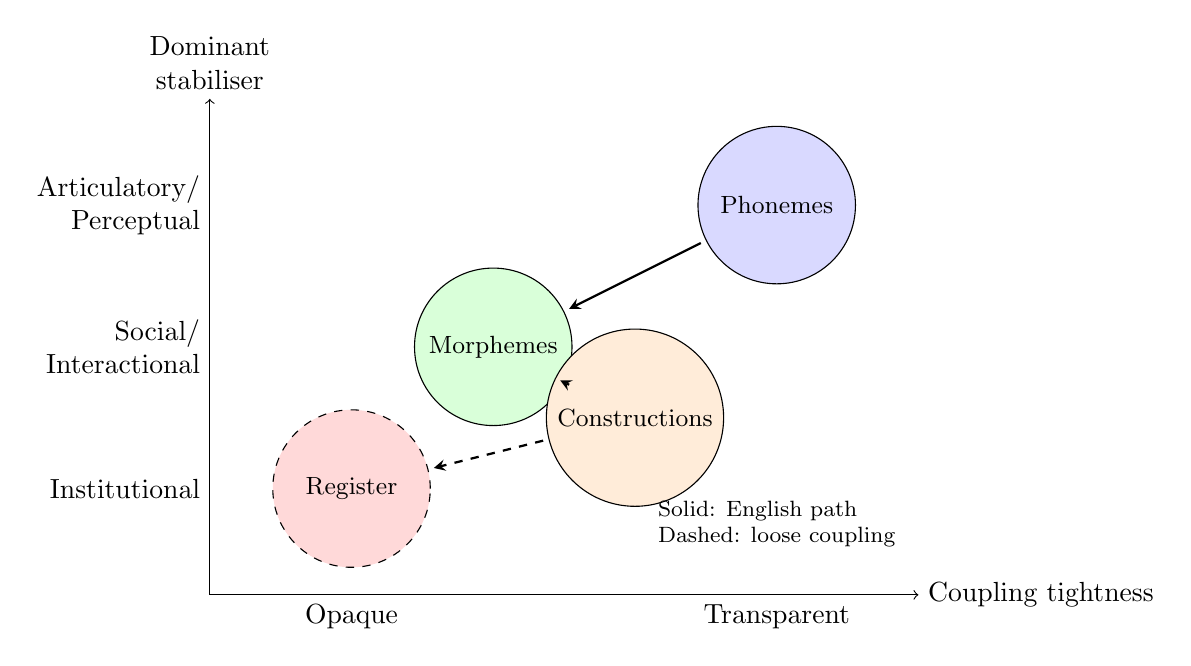
\begin{tikzpicture}[
    scale=0.9,
    tier/.style={circle, draw, minimum size=2cm, align=center, font=\small},
    arrow/.style={->, thick, >=stealth, shorten >=2pt, shorten <=2pt}
]

% Axes
\draw[->] (0,0) -- (10,0) node[right] {Coupling tightness};
\draw[->] (0,0) -- (0,7) node[above, align=center] {Dominant\\stabiliser};

% Axis labels
\node[below] at (2,0) {Opaque};
\node[below] at (8,0) {Transparent};
\node[left, align=right] at (0,1.5) {Institutional};
\node[left, align=right] at (0,3.5) {Social/\\Interactional};
\node[left, align=right] at (0,5.5) {Articulatory/\\Perceptual};

% English path (solid)
\node[tier, fill=blue!15] (phon) at (8,5.5) {Phonemes};
\node[tier, fill=green!15] (morph) at (4,3.5) {Morphemes};
\node[tier, fill=orange!15] (cxn) at (6,2.5) {Constructions};
\node[tier, fill=red!15, dashed] (reg) at (2,1.5) {Register};

\draw[arrow] (phon) -- (morph);
\draw[arrow] (morph) -- (cxn);
\draw[arrow, dashed] (cxn) -- (reg);

% Legend
\node[align=left, font=\footnotesize] at (8,1) {Solid: English path\\Dashed: loose coupling};

\end{tikzpicture}
\caption{Schematic illustration of the stabiliser-weighting map (not to scale). Different languages trace different paths through this space. An isolating language would compress the morpheme region; a polysynthetic language would expand it. The map is not a universal architecture but a tool for comparing coupling regimes.}
\label{fig:13:map}
\end{figure}

Three points about the figure:

\paragraph{It's a schematic, not data.} The positions are approximate. I don't have measures of ``coupling tightness''---the concept is qualitative. The figure is an illustration of the framework, not evidence for it.

\paragraph{The path is English-specific.} Other languages trace different paths. An isolating language like Vietnamese has a thin morpheme region; a polysynthetic language like Mohawk has a thick one that blurs into syntax. A click language like !Xóõ reorganises phonetic space in ways that shift the stabiliser weighting even at the sound level.

\paragraph{Register is dashed for a reason.} The connection between constructions and register is empirically weaker. Constructions are tight HPCs; register, as I'll argue in §\ref{sec:13:negative}, is not. The dashed line signals a different kind of relationship---institutional maintenance rather than homeostatic coupling.

%--- --- --- --- --- --- --- --- --- --- --- --- --- --- --- --- ---
\section{Cross-linguistic stress-test}
\label{sec:13:crossling}
%--- --- --- --- --- --- --- --- --- --- --- --- --- --- --- --- ---

\begin{formal}
The HPC explanatory strategy is domain-general. The stack itself is not universal.

\paragraph{Mohawk (polysynthetic).} A single Mohawk word can express what English requires a full sentence to express. The morpheme-word-clause boundaries that seem natural in English are blurred. Does the ``morpheme tier'' exist in Mohawk? Yes, but it's structured differently---incorporated nouns, complex verb templates, and applicative morphology reorganise the form--function couplings.

\paragraph{Vietnamese (isolating).} Vietnamese has minimal bound morphology. Tense, aspect, and mood are marked by particles or inferred from context. Is there a ``morpheme tier'' in the English sense? Barely. The stabiliser weighting shifts: storage mechanisms operate on particles and constructions rather than on bound affixes.

\paragraph{!Xóõ (click-heavy).} With over 100 phonemes including multiple click types, !Xóõ's phoneme inventory is stabilised by a different mechanism mix. Click production requires distinct articulatory coordination; click perception involves different cue weighting. The quantal-regions story from English doesn't transfer directly.

\textbf{Lesson:} Where the English cuts won't line up, the method still applies. Each language has its own stabiliser-weighting profile. The framework tells you what to look for; it doesn't prescribe what you'll find.
\end{formal}

%--- --- --- --- --- --- --- --- --- --- --- --- --- --- --- --- ---
\section{Negative cases: when the framework says no}
\label{sec:13:negative}
%--- --- --- --- --- --- --- --- --- --- --- --- --- --- --- --- ---

The HPC framework would be toothless if it said yes to everything. Here are three cases where it says no.

\subsection{Academic register}

Academic writing has a recognisable flavour. Passive constructions. Nominalisations. Hedges like \mention{it has been argued} and \mention{the data suggest}. Author-effacing expressions. You'd think this would be a natural category---a register, a style, maybe even a construction in the extended sense.

But watch what happens when you stress-test it.

Put the same researcher in front of a grant panel, a blog audience, and a conference poster. The passives evaporate. The hedges reweight. The nominalisations drop by half. The bundle doesn't resist perturbation; it dissolves and reconstitutes in a new configuration.

That's not homeostasis. The cluster doesn't cohere because there's no internal mechanism binding these features together. What holds them together is \emph{external}---genre conventions, disciplinary gatekeeping, editorial norms. Remove the external pressure, and the features scatter.

\paragraph{Diagnosis:} Academic register is a successful social institution, not a homeostatic property cluster. It's maintained by normative policing, not by cognitive binding. The HPC framework can describe this maintenance mode (I called it ``institutional'' in the stabiliser map), but it predicts exactly what we observe: rapid reweighting under perturbation, heterogeneous mechanisms, no stable internal geometry.

\subsection{``Indo-European''}

Indo-European is a language family---a genealogical grouping defined by historical descent. Languages are Indo-European because they descend from a common ancestor, not because mechanisms maintain their clustering.

Is Indo-European an HPC?

The cluster properties are real: cognate vocabulary, shared sound correspondences, similar grammatical patterns. But the mechanisms are historical (common origin), not homeostatic (ongoing maintenance). Modern English doesn't stay Indo-European because of stabilisers pushing it back toward the prototype. It's Indo-European because of where it came from.

\paragraph{Diagnosis:} Indo-European is a historical kind, not a homeostatic kind. The HPC framework doesn't apply---not because the category is illegitimate, but because the maintenance mode is different. Historical kinds are defined by causal continuity with an origin; homeostatic kinds are defined by mechanisms that maintain covariance.

(One might wonder: do prescriptive traditions constitute a homeostatic mechanism for Indo-European-ness? Perhaps for certain prestige forms, but not for the family as a whole. There's no pressure pushing English back toward Proto-Indo-European; if anything, the pressures push it away.)

\subsection{``Polysynthetic language''}

Polysynthetic languages are characterised by high morpheme-to-word ratios, incorporating structures, and complex verb templates. Mohawk, Ainu, and various Amerindian languages are standard examples.

Is ``polysynthetic'' an HPC?

The properties cluster---kind of. Polysynthetic languages do tend to have noun incorporation, applicatives, head-marking, and other features. But the clustering is loose. Languages are called polysynthetic if they score high on several dimensions, but the threshold is gradient and the dimensions don't cohere tightly.

More importantly, the mechanisms are heterogeneous. Why does Mohawk have noun incorporation? Historical and structural reasons specific to Iroquoian. Why does Ainu have complex verb templates? Different reasons specific to Ainu's history and structure. There's no single mechanism maintaining ``polysynthesis'' across the family.

\paragraph{Diagnosis:} Polysynthetic is a typological label, not a natural kind. It names a region in morphological space without implying that the region is carved by mechanisms. Different languages arrive at polysynthetic-like profiles by different routes; there's no convergent stabilisation.

\subsection{What the negative cases show}

These three cases---academic register, Indo-European, polysynthetic---fail the HPC diagnostics for different reasons:

\begin{itemize}
    \item \textbf{Academic register}: maintained by institutional policing, not cognitive binding. High looping intensity (the category changes because it's classified).
    \item \textbf{Indo-European}: maintained by historical continuity, not ongoing mechanisms. Not false, just a different kind of kind.
    \item \textbf{Polysynthetic}: a gradient label over heterogeneous structures. No stable mechanism profile.
\end{itemize}

The HPC framework can distinguish these failure modes. That's the payoff of having explicit diagnostics: you can say \emph{why} something doesn't qualify, not just that it doesn't.

%--- --- --- --- --- --- --- --- --- --- --- --- --- --- --- --- ---
\section{Looking forward}
\label{sec:13:forward}
%--- --- --- --- --- --- --- --- --- --- --- --- --- --- --- --- ---

This chapter has argued that the HPC explanatory strategy scales across linguistic levels. Phonemes, morphemes, and constructions are all homeostatic property clusters maintained by mechanisms. What differs is the coupling regime: transparent at the sound level, opaque at the morpheme level, architectural at the construction level.

But one level has special status.

Throughout the case studies in Part III---countability, definiteness, gender, lexical categories---the categories clustered at the morphosyntactic level. That's where form--function coupling is both \emph{tight} and \emph{obligatory}. You can speak without using \mention{let alone}. You can't speak without committing to count, tense, and definiteness.

Morphosyntax is the zone of maximum systematicity: the region of grammar where coupling is enforced, not optional. Chapter~\ref{ch:grammaticality-itself} asks what happens when we take this observation seriously. If grammaticality is what emerges when form--meaning coupling is obligatory, compositional, and learnable---then grammaticality itself is a kind. The deepest category in the stack.

\end{chapter}
